%
% The first command in your LaTeX source must be the \documentclass command.
\documentclass[sigconf]{acmart}
\definecolor{pblue}{rgb}{0.13,0.13,1}
\definecolor{pgreen}{rgb}{0,0.5,0}
\definecolor{pred}{rgb}{0.9,0,0}
\definecolor{pgrey}{rgb}{0.46,0.45,0.48}
\usepackage{tabularx}
\usepackage{listings}

\lstset{language=Java,
  showspaces=false,
  showtabs=false,
  breaklines=true,
  showstringspaces=false,
  breakatwhitespace=true,
  commentstyle=\color{pgreen},
  keywordstyle=\color{pblue},
  stringstyle=\color{pred},
  basicstyle=\ttfamily,
  moredelim=[il][\textcolor{pgrey}]{$$},
  moredelim=[is][\textcolor{pgrey}]{\%\%}{\%\%}
}

\def\code#1{\texttt{#1}}
\long\def\red#1{\textcolor{red}{#1}}

%
% defining the \BibTeX command - from Oren Patashnik's original BibTeX documentation.
\def\BibTeX{{\rm B\kern-.05em{\sc i\kern-.025em b}\kern-.08emT\kern-.1667em\lower.7ex\hbox{E}\kern-.125emX}}

% Rights management information.
% This information is sent to you when you complete the rights form.
% These commands have SAMPLE values in them; it is your responsibility as an author to replace
% the commands and values with those provided to you when you complete the rights form.
%
% These commands are for a PROCEEDINGS abstract or paper.
\copyrightyear{2018}
\acmYear{2018}
\setcopyright{acmlicensed}
\acmConference[LA WEB]{Woodstock '18: ACM Symposium on Neural Gaze Detection}{June 03--05, 2018}{Woodstock, NY}
\acmBooktitle{Woodstock '18: ACM Symposium on Neural Gaze Detection, June 03--05, 2018, Woodstock, NY}
\acmPrice{15.00}
\acmDOI{10.1145/1122445.1122456}
\acmISBN{978-1-4503-9999-9/18/06}

%
% These commands are for a JOURNAL article.
%\setcopyright{acmcopyright}
%\acmJournal{TOG}
%\acmYear{2018}\acmVolume{37}\acmNumber{4}\acmArticle{111}\acmMonth{8}
%\acmDOI{10.1145/1122445.1122456}

%
% Submission ID.
% Use this when submitting an article to a sponsored event. You'll receive a unique submission ID from the organizers
% of the event, and this ID should be used as the parameter to this command.
%\acmSubmissionID{123-A56-BU3}

%
% The majority of ACM publications use numbered citations and references. If you are preparing content for an event
% sponsored by ACM SIGGRAPH, you must use the "author year" style of citations and references. Uncommenting
% the next command will enable that style.
%\citestyle{acmauthoryear}

%
% end of the preamble, start of the body of the document source.
\begin{document}

%
% The "title" command has an optional parameter, allowing the author to define a "short title" to be used in page headers.
\title{After Brazil's General Data Protection Law: Authorization in Solid Web Apps}

%
% The "author" command and its associated commands are used to define the authors and their affiliations.
% Of note is the shared affiliation of the first two authors, and the "authornote" and "authornotemark" commands
% used to denote shared contribution to the research.
\author{Jefferson O. Silva}
\email{silvajo@pucsp.br}
\affiliation{%
  \institution{Pontifical Catholic University of S\~ao Paulo}
  \city{S\~ao Paulo}
  \country{Brazil}
}

\author{Newton Calegari}
\email{newton@nic.br}
\affiliation{%
  \institution{Brazilian Network Information Center - NIC.br}
  \city{S\~ao Paulo}
  \country{Brazil}
}

\author{Diogo Cortiz}
\affiliation{%
  \institution{Inria Paris-Rocquencourt}
  \city{S\~ao Paulo}
  \country{Brazil}
}

%
% By default, the full list of authors will be used in the page headers. Often, this list is too long, and will overlap
% other information printed in the page headers. This command allows the author to define a more concise list
% of authors' names for this purpose.
\renewcommand{\shortauthors}{Silva et al.}

%
% The abstract is a short summary of the work to be presented in the article.
\begin{abstract}
Write the abstract here.

\end{abstract}

%
% The code below is generated by the tool at http://dl.acm.org/ccs.cfm.
% Please copy and paste the code instead of the example below.
%
\begin{CCSXML}
<ccs2012>
 <concept>
  <concept_id>10010520.10010553.10010562</concept_id>
  <concept_desc>Computer systems organization~Embedded systems</concept_desc>
  <concept_significance>500</concept_significance>
 </concept>
 <concept>
  <concept_id>10010520.10010575.10010755</concept_id>
  <concept_desc>Computer systems organization~Redundancy</concept_desc>
  <concept_significance>300</concept_significance>
 </concept>
 <concept>
  <concept_id>10010520.10010553.10010554</concept_id>
  <concept_desc>Computer systems organization~Robotics</concept_desc>
  <concept_significance>100</concept_significance>
 </concept>
 <concept>
  <concept_id>10003033.10003083.10003095</concept_id>
  <concept_desc>Networks~Network reliability</concept_desc>
  <concept_significance>100</concept_significance>
 </concept>
</ccs2012>
\end{CCSXML}

\ccsdesc[500]{Computer systems organization~Embedded systems}
\ccsdesc[300]{Computer systems organization~Redundancy}
\ccsdesc{Computer systems organization~Robotics}
\ccsdesc[100]{Networks~Network reliability}

%
% Keywords. The author(s) should pick words that accurately describe the work being
% presented. Separate the keywords with commas.
\keywords{Solid, Access control, Decentralized web, Frameworks, Guardian}

%
% This command processes the author and affiliation and title information and builds
% the first part of the formatted document.
\maketitle

\section{Introduction}

With the approval of the Brazilian General Data Protection Law (LGPD),\footnote{http://www.planalto.gov.br/ccivil\_03/\_Ato2015-2018/2018/Lei/L13709.htm} several software companies may need to redesign the applications that handle the personal data of Brazilian citizens. LGPD considers personal any data that directly or indirectly lead to the identification of a user [\red{REF}]. Violations can lead to fines up to \red{2}\% of global revenue.

LGPD sets compliance requirements on the companies in charge of making decisions about the data processing (i.e., data controllers) and the companies that process personal data in the name of data controllers (i.e., data processors). LGPD states that, in some cases, data controllers and/or data processors may be held liable for any cause of action that involves harm to data subjects [\red{REF}].

To avoid being classified as either data processors or data controllers, some companies may redesign applications as decentralized Web Applications (Web Apps). \red{An application is considered decentralized when it does not hold users' data} [\red{REF}]. Tim Berners-Lee and colleagues [\red{REF}] propose a platform called Solid (derived from "\textbf{So}cial \textbf{li}nked \textbf{d}ata"), which can be described as a set of principles, conventions, and tools for building decentralized Web Apps. Solid is based on the principle that users should have full ownership of their data, which are stored in Web-accessible personal online datastores (pods). Pods are independent of Web Apps. For obtaining services, users need to authorize Web Apps to access their pods explicitly, by classifying Web Apps as trusted.

Nevertheless, this approach leaves users solely responsible for controlling access to protected resources, which may not be \linebreak enough to comply with the LGPD requirements of Privacy by Design. For example, a bank Web App may have an operation that reads personal data from the pods that should be accessible by account managers but not by analysts. A violation of this access control policy would configure a data breach, in which case the companies might be required to show that they applied appropriate controls, possibly from the software design.

\red{The current body of literature does not ...}

\vspace{0.15cm}
\noindent \textbf{RQ1: How decentralized Web Apps could be designed for privacy to comply with LGPD in an auditable fashion?}
\vspace{0.15cm}

The answer to our RQ may help companies...


\section{Background}
In this section, we offer some background on the Brazil's General Data Protection Law, on decentralized Web Apps in Solid, and on access control in Solid.

\subsection{Brazilian Data Protection Law}
The LGPD is strong inspired by the European GDPR. The Brazilian Bill, as the European one, defines cross-border jurisdiction, thus the Bill is applicable to any organizations processing personal data of Brazilian residents, whether it is headquartered in Brazil or not.

LGPD has also included the right of data portability, the right of access to personal data by the owner, and the right of erasure. Differently of the GDPR, which imposes 30 days for the controllers to comply with these requests, the LGPD imposes 15 days.

The Brazilian law also requires companies to nominate a Data Protection Officer (DPO) who will be in charge of monitoring the adoption of best practices for personal data protection and for reporting to the National Data Protection Authority (ANPD).

The regulation defines the concepts of personal data as "any data, isolated or aggregated to another, that may allow the identification of a natural person or subject them to a certain behavior" \cite{iapp2018}; sensitive data refers to data that may be subject to discriminatory practices, such as political opinion, sexual life, religious belief, genetic and biometric data, and it should have additional security layers; Unless it is possible to reverse-engineering the anonymized data, the law does not apply to this kind of data.

In a technical perspective, the efforts related to the decentralization of the Web help to build systems that are privacy-friendly, respecting user's privacy and in compliance with the regulations.

\subsection{Solid and the Decentralized Web}
Traditional social web applications, such as Facebook, Twitter, and others control its own data and have its own authentication and access control mechanisms, transforming them into centralized applications. In the contrast of this approach, there are emergent solutions proposing a new perspective to enable decoupling application logic and user data, allowing it to create privacy-friendly services on the Web.

Solid is a platform that supports decentralized social web applications, relying on open standards and on semantic web technologies. In the Solid platform, applications run in a browser or as mobile applications, while users` data are stored in a Web-accessible personal on-line data store (pod). Protocols for authentication, access control, communications among servers and applications are specified in the platform \cite{Sambra2016}.

Data used by applications built on top of Solid is stored in users` pods, while pods can be stored on pod servers. Pod servers manage data according to the Linked Data Platform recommendation, enabling it to manipulate data items through HTTP requests \cite{LDP}. Solid servers are, as defined by their authors \cite{Sambra2016},\linebreak application-agnostic, and can deal with both structured and unstructured data. The first is represented using RDF, a Semantic Web standard, and the latter is any type of data, such as videos, images, HTML web pages.

Application development based on (\red{in???}) Solid platform supports portability and interoperability, so applications can be seen as an interface that works with distributed data in multiple pod server implementations.

Identity in the Solid context is based on WebID, which allows agents (a person, an organization, etc.) to create their own identities using global unique identifiers - HTTP URIs \cite{Sambra2016solid}. WebID is an open and decentralized identification mechanism being developed by a W3C community group\footnote{\url{https://www.w3.org/community/webid/}}.

The main idea behind Solid is to put people back in control of their data, allowing them to choose where to store their own data. Solid proposal is aligned with the view of a \textit{decentralized web}, where data is decentralized and stored in personal data storage, or distributed servers in which the user has full control over its own data \cite{verborgh_iswc_2018}.

In a decentralized web model, resources created using one application can be read and modified by a different application without prior agreement between the applications. It is possible because the applications are interfaces to access data stored in multiple locations, such as in a \textit{pod}.

One can say that the decentralized web is characterized by \linebreak changing data ownership, giving users the tools to have full control of their data, supported by legal instruments, such as GDPR and LGPD, that empower them to control their own personal information.

\subsection{Access Control in Solid}

Access control is typically split into two distinct procedures: authentication, and authorization. While authentication is concerned with determining whether an agent (e.g., user, group) is whom it claims to be, authorization is responsible for verifying if the agent is allowed to access a protected resource (e.g., document) or operation (e.g., read, write, append).

The Solid project uses the Web Access Control (WAC) specification for controlling the access to protected resources. WAC specifies a decentralized cross-domain access control system, similar to existing access control models. According to the specification, WAC has the following key features:

\begin{enumerate}
\item The resources are identified by URLs and can refer to any web documents or resources.
\item It is declarative -- access control policies are written in regular web documents.
\item Users and groups are also identified by URLs (specifically, by WebIDs).
\item It is cross-domain -- all of its components, such as resources, agent WebIDs, and even the documents containing the access control policies, can potentially reside on separate domains.
\end{enumerate}

\begin{figure}
  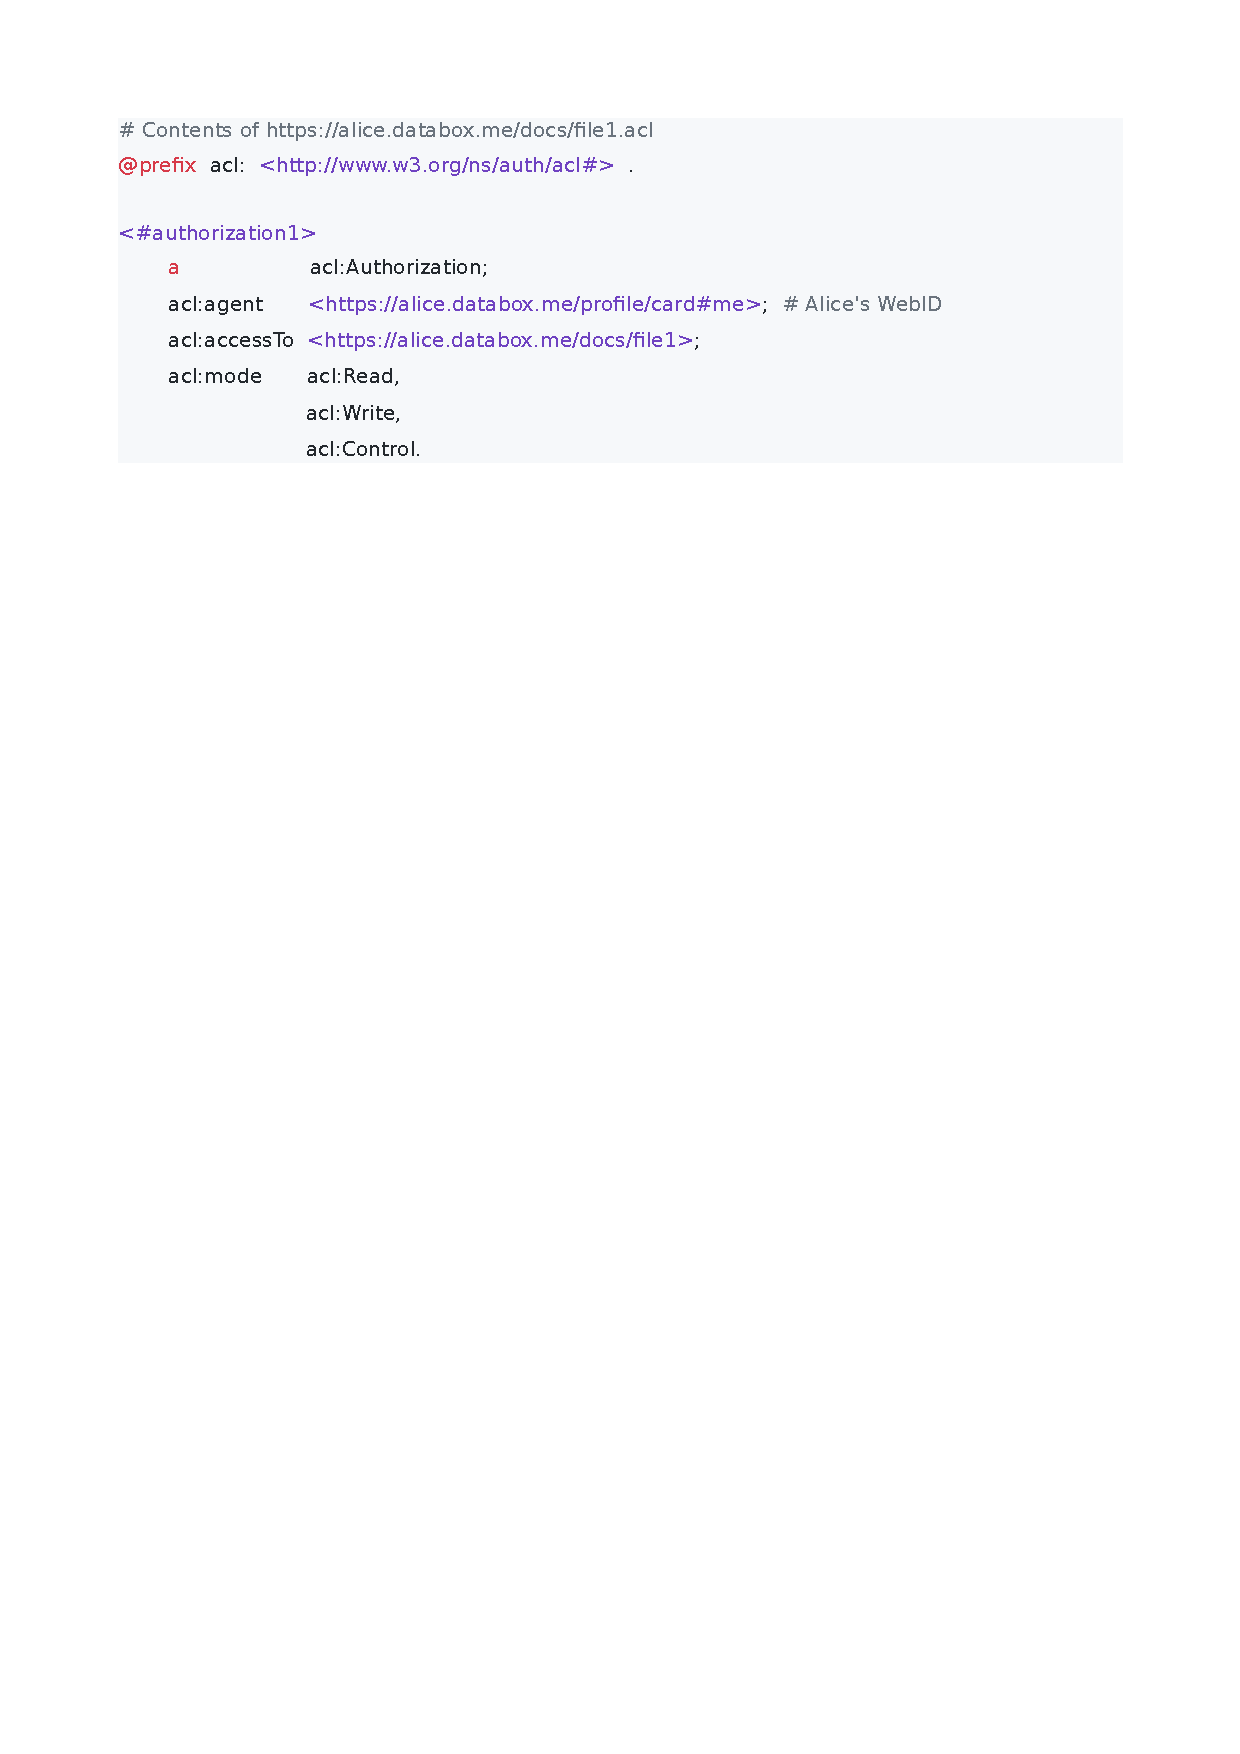
\includegraphics[trim=2cm 21.9cm 4.7cm 2cm, clip, scale=0.57]{pdf/alice-permission}
  \caption{Example WAC Document}
  \label{fig:individual-permission}
\end{figure}

Figure \ref{fig:individual-permission} shows an example of a WAC document that specifies that Alice (as identified by her WebID \code{https://alice.\\databox.me/profile/card\#me}) has full access (read, write, and control) to one of her web resources, located at \code{https://\\alice.databox.me/docs/file1}.


\begin{figure}
  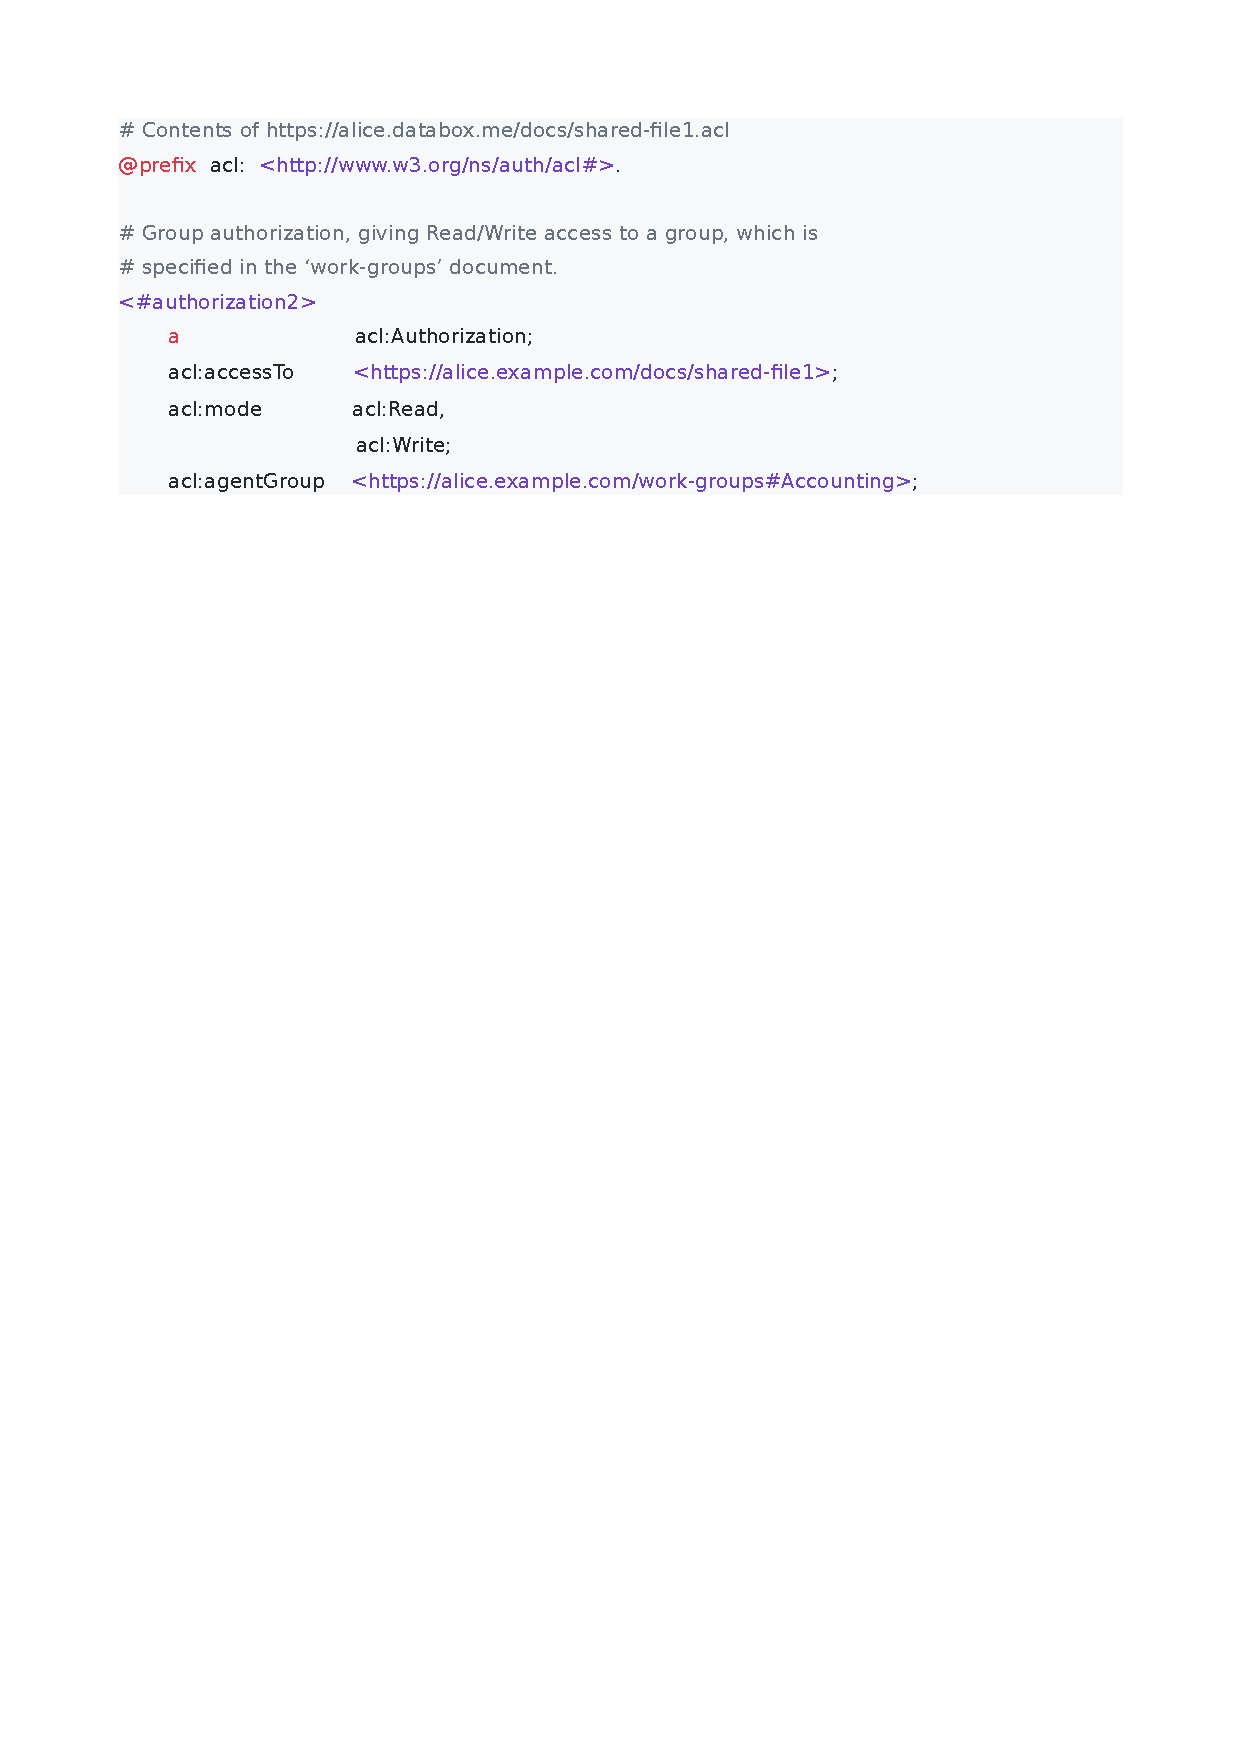
\includegraphics[trim=2cm 21.2cm 4.7cm 2cm, clip, scale=0.57]{pdf/shared-file1}
  \caption{WAC document with group permission}
  \label{fig:group-permission}
\end{figure}

In Figure \ref{fig:group-permission}, we can see that it is possible to give access to a group of agents using the \code{acl:agentGroup} predicate. A group is a collection of members (or WebIDs) that needs to be specified in a different file. In this case, members of the group \code{Accounting} can read and write the Alice's resource located \linebreak at \code{https://alice.example.com\//docs/shared-file1}.

Figure \ref{fig:group-listing} depicts the listing of a group. In this case, \code{Bob} and \code{Candice} belong to the \code{Accounting} group. Additionally, it is possible to give access to all agents (public access) or yet to all authenticated agents. It is also possible to classify web apps as trusted. Furthermore, not every document needs its own individual access control list file. Rather, it is possible to create an authorization to a container, which is a web location that contain multiple resources.

\begin{figure}
  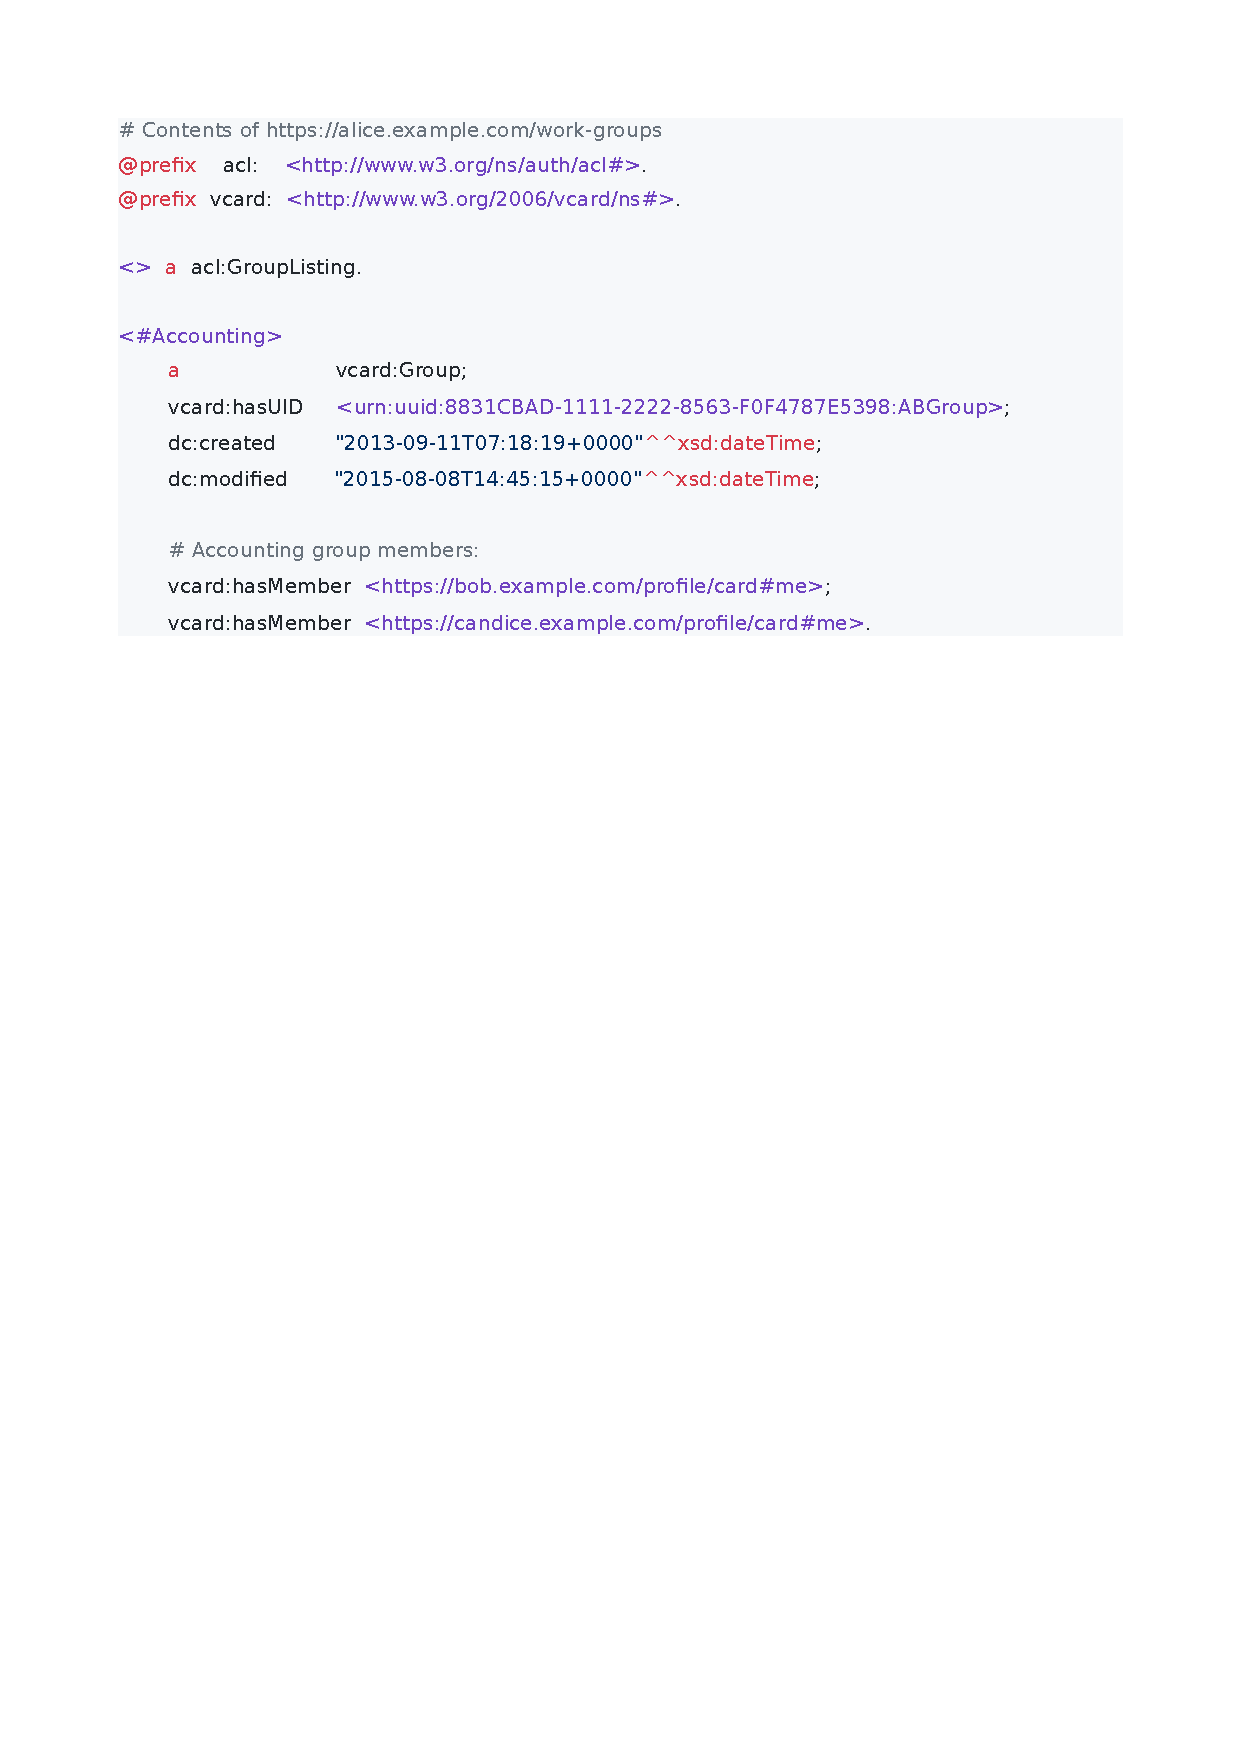
\includegraphics[trim=2cm 19cm 4.7cm 2cm, clip, scale=0.57]{pdf/work-groups}
  \caption{WAC document listing group members}
  \label{fig:group-listing}
\end{figure}


\subsection{Frameworks (temp)}
Guerra et al. \cite{Guerra2015}

\section{Esfinge Guardian}
In this section, we present the Esfinge Guardian\footnote{https://github.com/EsfingeFramework/guardian} framework. Essentially, the Esfinge Guardian framework is an intercepting mechanism between a requester and a protected operation. Figure \ref{fig:interception-mechanism} illustrates Guardian intercepting a requester's access to a protected operation on a resource.

\begin{figure}
  \centering
  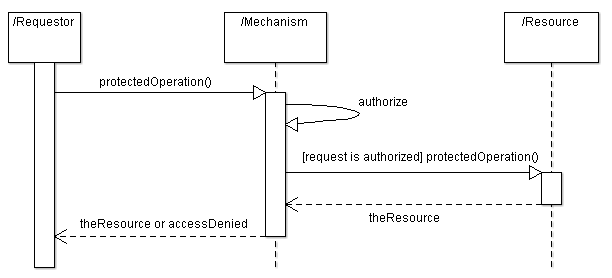
\includegraphics[scale=0.5]{img/interception-mechanism.png}
  \caption{A conceptualization of the interception mechanism. Silva et al. \cite{Silva2013}}
  \label{fig:interception-mechanism}
\end{figure}


As depicted in Figure \ref{fig:guardian-class-diagram}, Guardian is composed of eight main elements.







\noindent \verb|AuthorizationContext|. It is the central entity that holds all the information required for an authorization, which includes the data for the subject, resource, and environment. That means all other entities should provide AuthorizationContext with enough information for authorization to occur. It is also an interface with the user, meaning that all other points must be hidden from the user.

\noindent \verb|GuardianInterceptor|: is the entity responsible for abstracting the different existing interception technologies such as \linebreak aspect-orientation, CGLib, dynamic proxy etc.


\noindent \verb|Invoker|: is an entity with the ability to mimic the operation performed by the subject on a protected resource. In the Esfinge \linebreak Guardian framework, this element can execute methods; however, it is important to note that is just one of the possibilities since the architectural model is general.


\noindent \verb|Populator|: It is the entity that contains the data extraction logic for authorization. Information for authorization can be anywhere such as databases, files, shared variables, user session, arguments, Internet, etc. For this reason, Populator is an entity that knows how to obtain information from all these places.


\noindent \verb|PopulatorProcessor|: Entity that gathers and executes all defined Populators in the application.


\noindent \verb|Authorizer|: Entity that implements the logic of the access control policy and may use information stored in AuthorizationContext if necessary. There must be at least one Authorizer. Every Authorizer must provide its response to the AuthorizationProcessor, usually a "yes" or "no"; however, it must be possible to include other response types such as "Indeterminate".


\noindent \verb|AuthorizerProcessor|: Entity that contains the combining algorithm for all the Authorizers defined in the application.


\noindent \verb|AuthorizationMetada|: Entity that indicates which resources – or their operations – must be intercepted by the authorization mechanism. A requirement is that this element must be of metadata type, so that it can be used declaratively. Esfinge Guardian uses Java annotations as the implementation of this element; however, it can be considered a general marking element that is independent of a specific technology.



\begin{figure*}
  \centering
  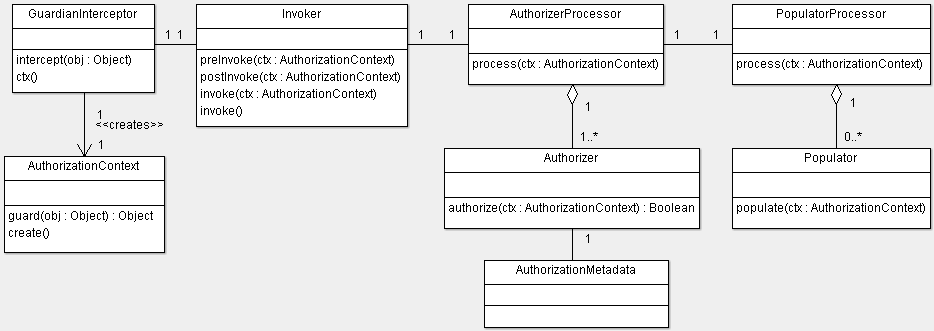
\includegraphics[scale=0.45]{img/guardian-class-diagram.png}
  \caption{Esfinge Guardian class diagram \cite{Silva2013}}
  \label{fig:guardian-class-diagram}
\end{figure*}



\section{Case Example}

\begin{lstlisting}

public class HierarchyAuthorizer
 implements Authorizer<RespectHierarchy> {

  public Boolean authorize(
                  AuthorizationContext c,
                    RespectHierarchy rh) {

  Set<String> roles = ctx.subject("roles");
  //retrieve other relevant information from ctx
  return //hierarchy authorization logic;
  }
}

\end{lstlisting}

\section{Discussion}

Here goes some discussion.

\section{Related Work}
The new regulations about data protection (i.e. GDPR, LGDP) bring new technical challenges related to how applications will handle personal data still be in compliance the law in terms of privacy. Application vendors are already able to guarantee compliance to these regulations in their tools in terms of consent management and personal data tracking, although data portability and interoperability among different products and services are still big challenges to tackle.

According to \cite{bonatti2018data}, it is necessary to have tools and best practices to help building privacy-by-design systems\cite{cavoukian2009privacy}. Authors argue that the standardization work in this domain still have to address the interoperability challenge. There are no standard ontology that align the terminology of privacy legislation with vocabularies to describe and interchange data, thus enabling personal data portability.

There are ongoing initiatives putting together efforts to develop vocabularies and standards to enable semantic interoperability and transparency logs about personal data processing. A primary forum working on this matter is the 'W3C Community Group' entitled \textit{Data Privacy Vocabularies and Controls CG}.

Performance is an issue in the decentralization model\cite{verborgh_iswc_2018}. The heterogeneity and distribution of a decentralized network implies that data processing algorithms will require more computational resources to perform tasks, comparing it with the centralized ones.

Author points out that federated SPARQL query engines perform better in private networks instead of on the public Web. Thus, a suitable alternative to overcome this issue is the promising \linebreak \textit{Linked Data Fragments}\cite{LDF}, less expressive query interfaces. 

\section{Conclusion}
Here goes a conclusion.


\section{BACKUP}
1.%%  NEW PROPOSITION OF PARAGRAPH%%
LGPD is based on the General Data Protection Regulation (GDPR),\footnote{http://data.consilium.europa.eu/doc/document/ST-9565-2015-INIT/en/pdf} which aims at protecting the personal data of EU individuals. In total, around 120 countries adopt comprehensive privacy laws and regulations to protect personal data held by private and public bodies \cite{Banisar2011}.



%
% The acknowledgments section is defined using the "acks" environment (and NOT an unnumbered section). This ensures
% the proper identification of the section in the article metadata, and the consistent spelling of the heading.
\begin{acks}
To the Brazilian Network Information Center (NIC.br) and to the Web Technologies Study Center (Ceweb.br) for maintaining a sustainable ecosystem to promote initiatives to keep the Internet and the Web open and accessible for everyone.
\end{acks}

%
% The next two lines define the bibliography style to be used, and the bibliography file.
\bibliographystyle{ACM-Reference-Format}
\bibliography{laweb19}


\end{document}
